\parttitle{VI}{Renewable-Energy and Climate Data: Catalogue and Analysis}

\section{Why this application domain}
\label{sec:why-energy}

Renewable-energy and climate series are the right proving ground for QRC for
reasons that survive scrutiny. The tasks are \emph{temporal} with memory and
nonlinearity at many scales --- cloud advection in minutes, weather synoptics
in days, seasonality in months, ENSO in years --- exactly the structure
reservoirs exist to exploit. The economic stakes are real and quantified:
grid operators price forecast error directly, and the classical forecasting
literature is mature enough to supply honest
baselines~\citep{inman2013solar,yang2018history,hong2016load,foley2012wind}.
The data are public, long, and well documented (Table~\ref{tab:datasets}).
And the problem class connects to genuine scientific frontiers --- data-driven
weather models now rival numerical weather prediction
\citep{rasp2020weatherbench,lam2023graphcast}, and classical reservoir
computing already operates at global-atmosphere scale
\citep{pathak2018model,arcomano2020machine} --- so quantum variants inherit a
meaningful yardstick rather than a toy one.

The QRC-and-adjacent record on these problems, read with Part~VIII's
discipline, is early but concrete. Hybrid quantum--classical reservoirs have
modelled thermal convection and two-dimensional Rayleigh--B\'enard turbulence
--- the fluid-dynamical core of weather --- in simulation
\citep{pfeffer2022hybrid,pfeffer2023reduced}. The recurrence-free QRC of
\citet{ahmed2024prediction} targets chaotic dynamics and \emph{extreme-event}
prediction, the tail-risk problem that dominates both grid operations and
climate adaptation, with shot-optimal training developed in
\citet{ahmed2025optimal}. Short-term load forecasting with gate-model QRC on
simulated IBM backends reports competitive accuracy at few-qubit scale on
real Moroccan-grid-adjacent data \citep{odo2026quantum}; wind-power
prediction has been benchmarked with quantum neural networks across feature
maps and ans\"atze \citep{hangun2025qnn,hangun2025comparative}. Perspective
pieces map where quantum computation could and could not matter for weather
and climate \citep{tennie2022quantum} and for power systems generally
\citep{ajagekar2019quantum,zhou2022quantum}. None of these works establishes
quantum advantage; collectively they establish feasibility, define tasks,
and --- read critically --- exhibit most of the benchmarking pitfalls Part~VIII
catalogues.

\section{Dataset catalogue}
\label{sec:catalogue}

Table~\ref{tab:datasets} catalogues twelve public datasets spanning the
domain. Selection criteria: documented provenance and licence, machine-readable
access, length sufficient for chronological train/validation/test splits, and
a live classical benchmark literature. The ``QRC suitability'' column encodes
this document's judgement of where each dataset meets current quantum
reservoirs --- which, per Parts~IV--V, means \emph{low-dimensional inputs}
(scalar-to-few channels; high-dimensional fields need aggressive classical
reduction first), \emph{thousands of time steps} (enough for honest splits
but within shot budgets), and targets where \emph{memory and nonlinearity},
not raw dimensionality, carry the difficulty.

\begin{table*}[tp]
\centering\scriptsize
\caption{Public datasets for renewable-energy and climate QRC studies.
Licences paraphrase the provider's terms; verify before redistribution.
``Resolution'' is temporal $\times$ spatial where applicable.}
\label{tab:datasets}
\setlength{\tabcolsep}{3pt}
\begin{tabular}{@{}p{2.5cm}p{1.5cm}p{3.1cm}p{2.2cm}p{2.3cm}p{3.4cm}@{}}
\toprule
Dataset (ref.) & Domain; licence & Variables; resolution & Size; span & Missing data; benchmark use & Preprocessing; QRC suitability \\
\midrule
NSRDB \citep{sengupta2018nsrdb} & solar; open (attrib.) & GHI/DNI/DHI, met.\ fields; 30\,min $\times$ 4\,km, CONUS+ & TB-scale; 1998-- & gap-filled product; solar-forecast standard & site extraction; clear-sky index (Eq.~\ref{eq:kt}); \textbf{high} for univariate $k_t$ tasks \\
SURFRAD \citep{augustine2000surfrad} & solar (ground truth); open & broadband radiation suite; 1--3\,min, 7 US sites & GB; 1995-- & instrument gaps flagged; validation standard & QC flags; averaging; \textbf{high} for minute-scale ramp studies \\
WIND Toolkit \citep{draxl2015wind} & wind; open & wind speed/power at hub heights; 5\,min $\times$ 2\,km & TB-scale; 2007--2013 & modelled (WRF) --- no sensor gaps; wind standard & site extraction; power-curve mapping; \textbf{medium} (modelled data caveat) \\
GEFCom2014 \citep{hong2016gefcom} & load/price/ solar/wind; research use & hourly load, temperature stations; task-defined & MB--GB; 2005--2011 & organiser-cleaned; probabilistic-forecast standard & pinball-loss targets; \textbf{high} for load track (used as template here) \\
UCI Electricity- LoadDiagrams \citep{trindade2015electricity} & load; open (CC-BY) & 370 client loads; 15\,min & 140\,MB; 2011--2014 & zeros before client onboarding & client selection; resample; \textbf{high}; standard in deep-forecasting papers \\
ENTSO-E Transparency \citep{hirth2018entsoe} & grid; free account & load, generation by fuel, prices; 15--60\,min, per zone & GB-scale; 2015-- & reporting gaps by TSO & API pulls; zone selection; \textbf{high} for national-load tasks \\
OPSD \citep{wiese2019open} & power system; open & curated ENTSO-E$+$weather packages; hourly & GB; 2015--2020 & documented per package & direct CSV; \textbf{high}; lowest-friction European option \\
Grid stability \citep{arzamasov2018towards} & grid dynamics; open (UCI) & 4-node DSGC simulation, 11 features $+$ label & 10\,k rows; static & none (synthetic) & classification target; \textbf{medium}: not a time series, useful for feature-map studies \\
Battery degradation \citep{severson2019data,saha2007battery} & storage; open & cycling curves, capacity, impedance & GB; 124 cells / NASA packs & protocol-dependent & cycle summarisation; \textbf{medium}: long-horizon regression, slow ``time'' axis \\
ERA5 \citep{hersbach2020era5} & weather/climate reanalysis; open (CDS) & full atmospheric state; hourly $\times$ 31\,km global & PB-scale; 1940-- & complete (reanalysis) & variable/level/site extraction; \textbf{medium}: needs reduction to few channels \\
Jena weather \citep{jena2026weather} & weather (site); open & 14 met.\ variables; 10\,min & 100\,MB-scale; 2003-- & short sensor gaps & resample; \textbf{high}: the standard small multivariate testbed \\
CMIP6 \citep{eyring2016cmip6} & climate projections; open (per-model) & multi-model fields, scenarios; monthly/daily & PB-scale; 1850--2100 & complete (model) & index extraction (e.g.\ Ni\~no 3.4); \textbf{low--medium}: distribution-shift studies \\
\bottomrule
\end{tabular}
\end{table*}

\section{Three datasets in depth}
\label{sec:deep-dives}

Three series carry the document's experiments: a solar irradiance series and
a system-load series --- both \emph{surrogates}, generated by
\code{datasets.py} to the statistical template of their public archetypes
(NSRDB-like and GEFCom-like respectively) so that this document is
self-contained, licence-clean, and exactly reproducible --- and the \emph{real}
monthly ENSO sea-surface-temperature record. Every statistic and figure below
is computed by \code{eda.py} from the shipped generators; the surrogate label
is repeated wherever a number could otherwise be mistaken for a measurement
of the physical world.

\subsection{Solar irradiance (surrogate, NSRDB-like)}
\label{sec:solar-dive}

\emph{Construction.} One year of 30-minute global horizontal irradiance (GHI)
at a low-latitude site ($1.35^\circ$N): a deterministic Haurwitz clear-sky
curve modulated by a two-state Markov cloud regime (clear/cloudy) with
Beta-distributed clear-sky index within regime, monsoon-season occupancy
modulation, and $2\%$ of daytime points removed in contiguous blocks to
emulate sensor outages.

\emph{The forecasting variable.} Solar work forecasts not GHI but the
\emph{clear-sky index}
\begin{equation}
  k_t \;=\; \frac{\mathrm{GHI}}{\mathrm{GHI}_{\mathrm{clear}}},
  \label{eq:kt}
\end{equation}
which removes the deterministic solar geometry that would otherwise dominate
every error metric~\citep{inman2013solar,yang2018history}; predicting GHI
directly and reporting low errors is the domain's classic self-deception, and
the persistence baseline must be applied to $k_t$, not GHI.

\emph{Statistics (daytime, elevation $>5^\circ$; $n=8286$).} GHI: mean
$461$, s.d.\ $292$, median $425$, $5$th/$95$th percentiles $64/908$, maximum
$1041$ (all $\mathrm{W\,m^{-2}}$), skewness $0.15$. Clear-sky index: mean
$0.72$, s.d.\ $0.28$, median $0.87$, skewness $-0.93$ --- the strong left skew
and the mass near $k_t\!\approx\!0.9$-$1.0$ are the bimodal
clear/cloudy signature that makes the series regime-switching rather than
smoothly stochastic. Missing data: $273$ daytime points ($1.6\%$), longest
gap $11$ steps ($5.5$ h) --- long enough that naive interpolation would
fabricate a whole afternoon; the pipeline masks rather than fills.

\emph{Temporal structure (Figure~\ref{fig:eda-solar}).} The daytime-only
autocorrelation of $k_t$ decays within a few hours --- memory is short and
regime-bound. The Welch spectrum of GHI shows the harmonic comb of the
diurnal cycle (24, 12, 8\,h lines) atop a broadband cloud continuum; after
the $k_t$ transform the comb collapses, which is the quantitative content of
Eq.~\eqref{eq:kt}. Implications for reservoir design: short usable memory
(small $\mathrm{MC}$ requirement), strong conditional heteroscedasticity
(regime transitions are where errors concentrate), and near-persistent
behaviour at 30-minute horizons --- which is why Part~IV's honest table shows
persistence so hard to beat, and why value, if any, lives at ramp events and
longer horizons.

\begin{figure*}[t]
\centering
\begin{subfigure}{0.495\textwidth}
  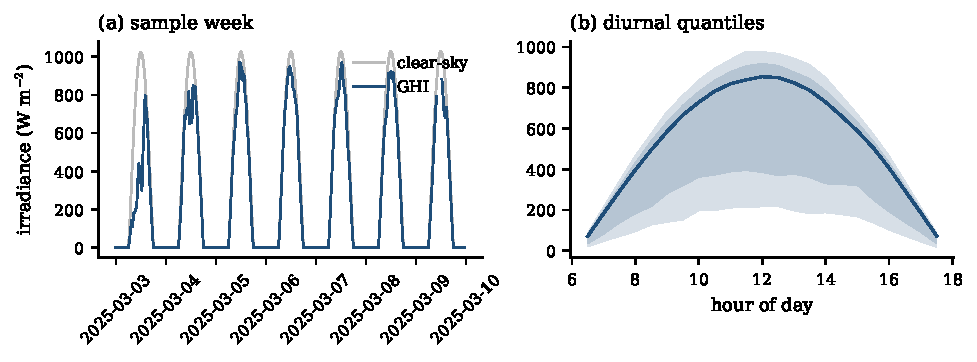
\includegraphics[width=\linewidth]{figures/eda_solar_overview.pdf}
\end{subfigure}\hfill
\begin{subfigure}{0.495\textwidth}
  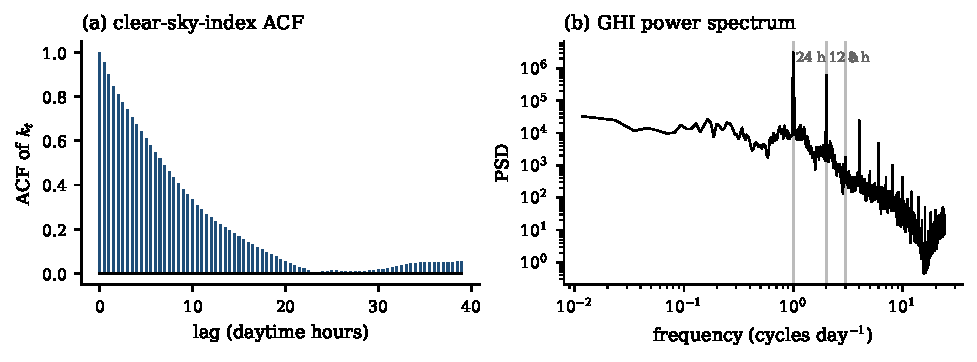
\includegraphics[width=\linewidth]{figures/eda_solar_stats.pdf}
\end{subfigure}
\caption{Solar surrogate EDA (from \code{eda.py}). Left pair: a sample week
of GHI against the clear-sky curve, and the diurnal quantile fan. Right
pair: daytime autocorrelation of $k_t$, and the GHI Welch spectrum with
diurnal harmonics marked. Simulation on surrogate data.}
\label{fig:eda-solar}
\end{figure*}

\subsection{System load (surrogate, GEFCom-like)}
\label{sec:load-dive}

\emph{Construction.} Three years of hourly system load: a double-peaked
diurnal profile, weekday/weekend distinction (weekend factor $0.86$), annual
seasonality, a linear cooling-degree-day (CDD) temperature response of
$55\,\mathrm{MW/^\circ C}$ above the comfort threshold, AR(1) residuals, and
eleven holiday days per year at factor $0.88$.

\emph{Statistics.} Mean $4280$\,MW, s.d.\ $542$, range $2647$--$5618$,
skewness $-0.10$; correlation with coincident temperature $0.64$ and with CDD
$0.63$ --- the canonical load--weather coupling that makes exogenous inputs
mandatory for competitive load
forecasting~\citep{hong2016load,hong2016gefcom}.

\emph{Temporal structure (Figure~\ref{fig:eda-load}).} The autocorrelation
shows the double comb at $24$\,h and $168$\,h --- daily and weekly cycles ---
persisting essentially undamped across the eight-day window: load is the
opposite of solar, a \emph{long-memory, strongly periodic} series where
calendar features do most of the work and the residual after calendar and
temperature is the actual forecasting problem. The correlation heat map
(load, lags, temperature, CDD, calendar flags) quantifies the redundancy a
read-out must negotiate. Implications: multivariate encoding (load lag,
temperature, calendar) rather than scalar; memory requirements modest
\emph{after} the calendar is handled classically; the correct QRC posture is
hybrid --- quantum features for the weather-driven residual, classical
features for the calendar --- exactly the Part~VII pipeline.

\begin{figure*}[t]
\centering
\begin{subfigure}{0.495\textwidth}
  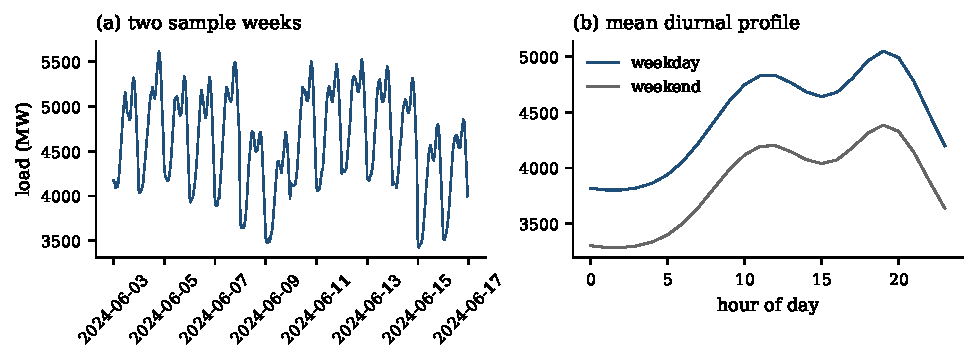
\includegraphics[width=\linewidth]{figures/eda_load_overview.pdf}
\end{subfigure}\hfill
\begin{subfigure}{0.495\textwidth}
  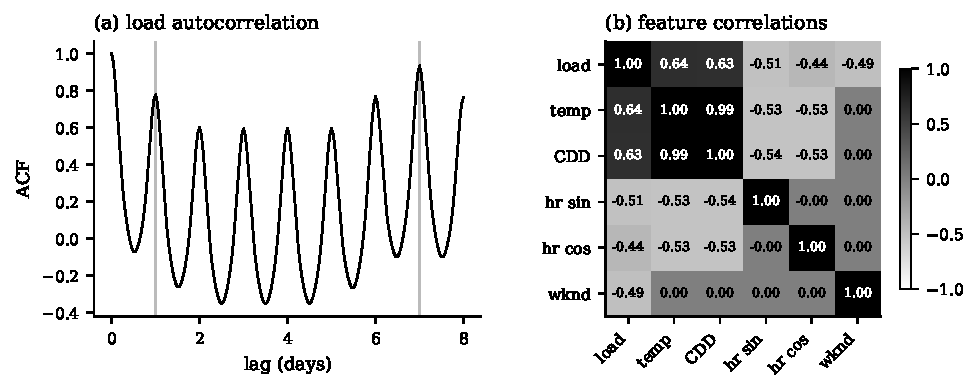
\includegraphics[width=\linewidth]{figures/eda_load_stats.pdf}
\end{subfigure}
\caption{Load surrogate EDA. Left pair: two sample weeks, and weekday versus
weekend diurnal profiles. Right pair: autocorrelation over eight days with
daily/weekly lags marked, and the feature correlation matrix. Simulation on
surrogate data.}
\label{fig:eda-load}
\end{figure*}

\subsection{ENSO sea-surface temperature (real data)}
\label{sec:enso-dive}

\emph{Provenance.} Monthly Ni\~no-region sea-surface temperature, 1950--2010
($n=732$), the NOAA record as bundled with \code{statsmodels}; anomalies are
computed against the monthly climatology, removing the seasonal cycle. This
is the one fully real series in the experiments, and the one with genuine
climate-dynamics content: ENSO is the dominant mode of interannual
variability, with delayed-oscillator dynamics --- coupled ocean--atmosphere
feedback with wave-transit delays --- giving it intrinsic memory and weak
chaos~\citep{suarez1988delayed}.

\emph{Statistics.} SST mean $23.09\,^\circ$C, s.d.\ $2.25$, range
$18.95$--$29.24$. Anomaly: s.d.\ $1.08\,^\circ$C, range $-2.43$ to $+4.60$,
skewness $+1.15$ --- the positive skew is physical (El Ni\~no warm events run
hotter than La Ni\~na events run cold) and any model evaluated only on MSE
will under-serve exactly the strong-event tail that matters.

\emph{Temporal structure (Figure~\ref{fig:eda-enso}).} The anomaly
autocorrelation decays over roughly $12$--$18$ months with a weak negative
lobe near $24$ months --- the oscillator signature; the variance-preserving
spectrum $f\,S(f)$ concentrates power in the $2$--$7$ year ENSO band.
Implications: memory of a year-plus is \emph{required}, which is precisely
why the windowed ($L=8$ months) feature map of Part~IV loses to the recurrent
reservoir here and why this series, small as it is, is the document's
sharpest architectural discriminator. The known hard cases --- the
spring predictability barrier, event-magnitude asymmetry --- make ENSO
indices a permanently honest benchmark: decades of classical effort define
what ``good'' means.

\begin{figure*}[t]
\centering
\begin{subfigure}{0.495\textwidth}
  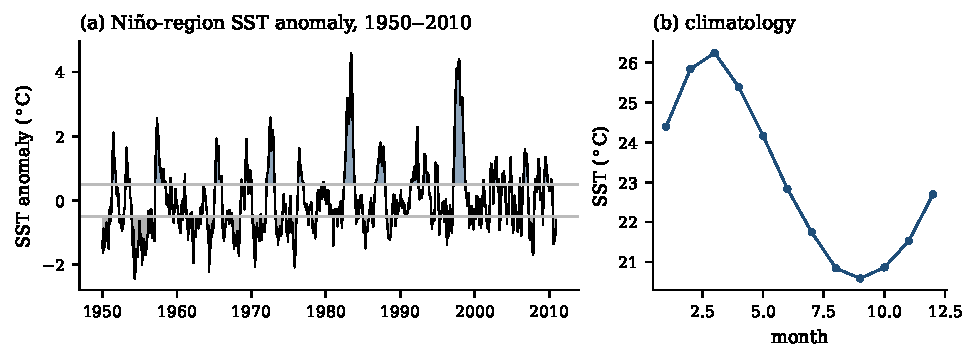
\includegraphics[width=\linewidth]{figures/eda_enso_overview.pdf}
\end{subfigure}\hfill
\begin{subfigure}{0.495\textwidth}
  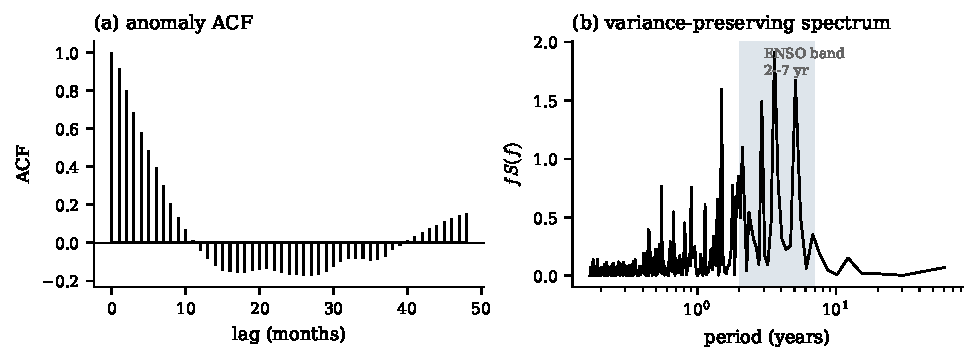
\includegraphics[width=\linewidth]{figures/eda_enso_stats.pdf}
\end{subfigure}
\caption{ENSO EDA (real data). Left pair: the anomaly series with
$\pm0.5\,^\circ$C event shading, and the monthly climatology. Right pair:
anomaly autocorrelation over 48 months, and the variance-preserving spectrum
with the 2--7-year band marked.}
\label{fig:eda-enso}
\end{figure*}
